%! Author = paulsenik
%! Date = 07.11.23

\begin{frame}{Linux}
    \section{Linux}\label{sec:Linux}
\end{frame}

\begin{frame}{Was ist Linux?}
    \subsection{Linux?}\label{subsec:linux?}

    \begin{quote}<2->
        \href{https://de.wikipedia.org/wiki/Linux}{Als GNU/Linux bezeichnet man in der Regel freie, unixähnliche Mehrbenutzer-Betriebssysteme, die auf dem Linux-Kernel und wesentlich auf GNU-Software basieren.}
    \end{quote}

    \begin{itemize}
        \item<3-> 1991 als Alternative zu UNIX erschaffen
        \item<4-> Freie und offene Alternative zu Windows und MacOS
        \item<5-> Unterstützung von großen Unternehmen (Google, Microsoft, Facebook, etc.)
    \end{itemize}
    \vspace{0.5cm}
    \begin{exampleblock}<1->{Fun Fact}
        Linux ist das größte Softwareprojekt der Welt.
    \end{exampleblock}

\end{frame}

\begin{frame}{Warum Linux?}
    \subsection{Warum Linux?}\label{subsec:warum-linux?}

    \begin{itemize}
        \item<2-> Performance und Stabilität
        \item<3-> Mehr Transparenz und Flexibilität durch OpenSource
        \item<4-> Sicherheit und Datenschutz (Keine Telemetriedaten)
    \end{itemize}
    \vspace{0.5cm}

    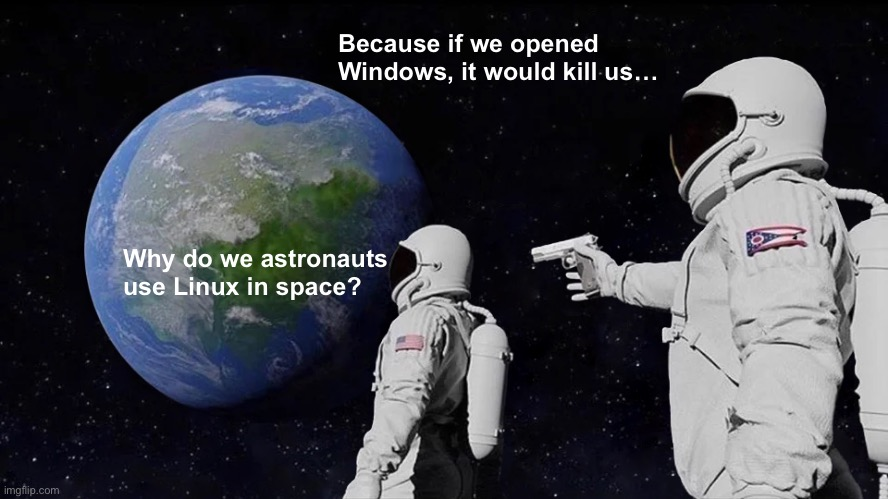
\includegraphics[width=7cm]{Meme_Space-Linux}
    \begin{exampleblock}<1->{Fun Fact}
        Linux im Weltall: ISS (Seit 1988) \& SpaceX (seit 2020).
    \end{exampleblock}

\end{frame}

\begin{frame}{Warum kein Linux?}
    \subsection{Warum kein Linux?}\label{subsec:warum-kein-linux?}

    \begin{itemize}
        \item<2-> Kein "Drop-In" Microsoft-Office-Ersatz
        \item<3-> Wenn man es einfach haben will (Man kann sehr viel Tüfteln)
        \item<4-> Mögliche Probleme bei komplexen Anwendungen, die nicht auf Linux zugeschnitten sind (Video-Bearbeitung, Spiele, ..)
    \end{itemize}

    \vspace{0.5cm}
    \begin{exampleblock}{Fun Fact}<1->
        \href{https://gs.statcounter.com/os-market-share/desktop/worldwide}{Linux läuft auf 4,5\% aller Privatrechner. (+ 2,25\% Chrome OS)}
    \end{exampleblock}

\end{frame}

\begin{frame}{Distributionen}
    \subsection{Distributionen}\label{subsec:distributionen}

    \begin{quote}<2->
        Eine Distribution ist ein Softwarepaket, dass auf dem Linux-Kernel aufbaut.
    \end{quote}

    \begin{itemize}
        \item[]<3-> Ein Großteil der Linux-Distributionen ist Teil dieser 3 "Familien":
    \end{itemize}

    \begin{itemize}
        \item<4-> Arch
        \item<5-> Debian $\longrightarrow$ Ubuntu
        \item<6-> RHEL (Red Hat Enterprise Linux)
    \end{itemize}

    \vspace{0.5cm}
    \begin{exampleblock}<1->{Fun Fact}
        Eine Distribution wird oft auch als "Distro", "Flavor" oder "Sorte" bezeichnet
    \end{exampleblock}

\end{frame}


\begin{frame}{Desktop Umgebungen}
    \subsection{Desktop Umgebungen}\label{subsec:desktop-umgebungen}

    \pause

    \begin{quote}
        \href{https://de.wikipedia.org/wiki/Desktop-Umgebung}{Eine Desktop-Umgebung ist eine grafische Arbeits- bzw. Benutzerumgebung von Betriebssystemen[\ldots]}
    \end{quote}

    \pause

    \begin{itemize}
        \item Desktops sind auch nur eigenständige Software in einer Linux-Distribution\pause
        \item Leicht (nach-)installierbar\pause
        \item Unterscheiden sich in:\pause
        \begin{itemize}
            \item Aussehen\pause
            \item Anpassbarkeit\pause
            \item Workflow-Möglichen
        \end{itemize}
    \end{itemize}

\end{frame}

\begin{frame}{Beispiele}
    \subsubsection{Beispiele}\label{subsubsec:beispiele}

    \href{https://opensource.com/article/20/5/linux-desktops}{Umfrage 2020}

    \begin{itemize}
        \item<2-> KDE Plasma (32\%)
        \item<3-> Gnome (24\%)
        \item<4-> XFCE (12\%)
        \item<5-> Cinnamon (11\%)
        \item<6-> sonst (21\%)
    \end{itemize}

    \vspace{0.5cm}
    \begin{exampleblock}<1->{Fun Fact}
        Die 500 schnellsten Supercomputer der Welt laufen auf Linux
    \end{exampleblock}

\end{frame}

\begin{frame}{KDE Plasma}
    \subsubsection{KDE Plasma}\label{subsubsec:KDE-Plasma}

    \begin{tikzpicture}
        [remember picture, overlay, shift={(current page.north east)}]
        \node[anchor=north east,xshift=-.3cm,yshift=-2cm]{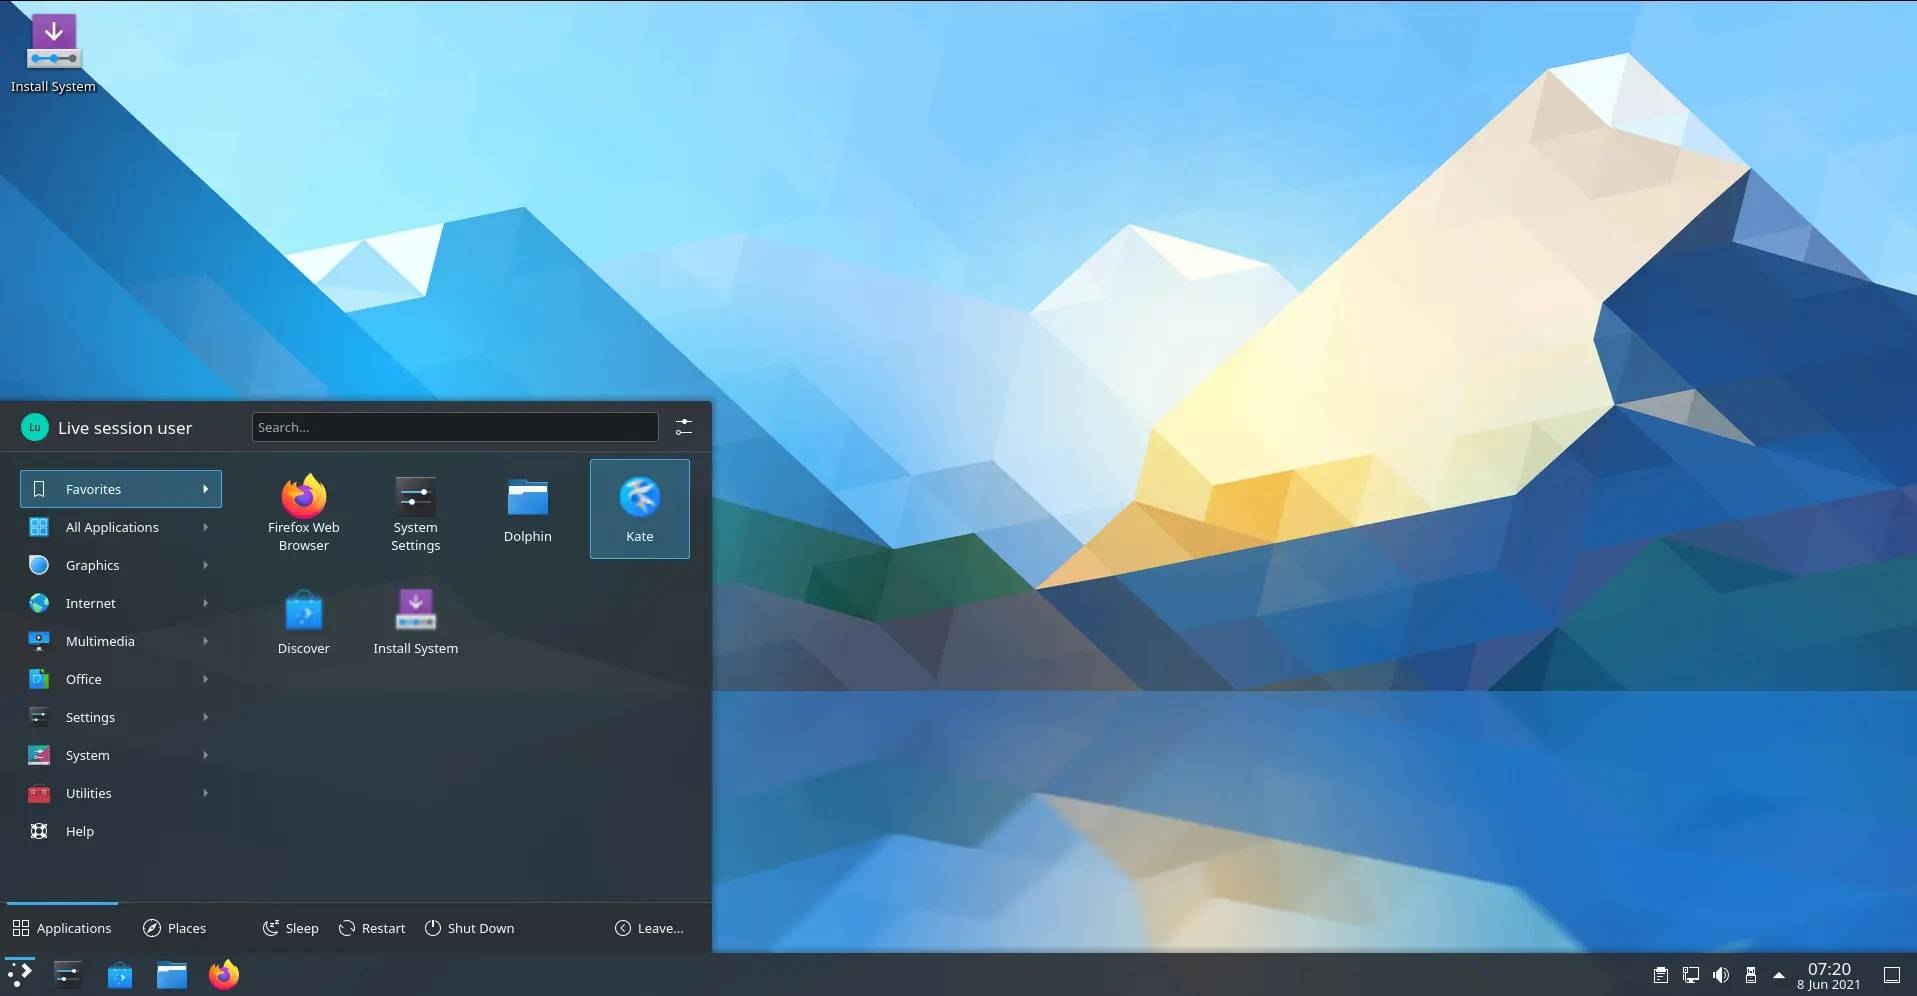
\includegraphics[width=12cm]{KDE-Plasma-Desktop}};
    \end{tikzpicture}

\end{frame}

\begin{frame}{Gnome}
    \subsubsection{Gnome}\label{subsubsec:Gnome}

    \begin{tikzpicture}
        [remember picture, overlay, shift={(current page.north east)}]
        \node[anchor=north east,xshift=-0.3cm,yshift=-1.7cm]{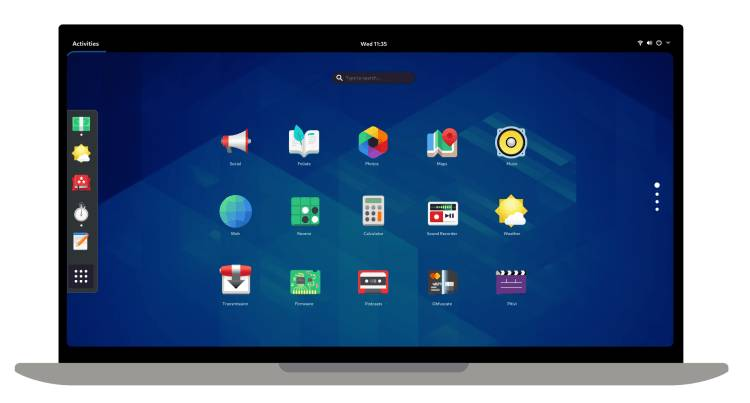
\includegraphics[width=12cm]{Gnome-Desktop}};
    \end{tikzpicture}

\end{frame}

\begin{frame}{XFCE}
    \subsubsection{XFCE}\label{subsubsec:XFCE}

    \begin{tikzpicture}
        [remember picture, overlay, shift={(current page.north east)}]
        \node[anchor=north east,xshift=-0.3cm,yshift=-1.7cm]{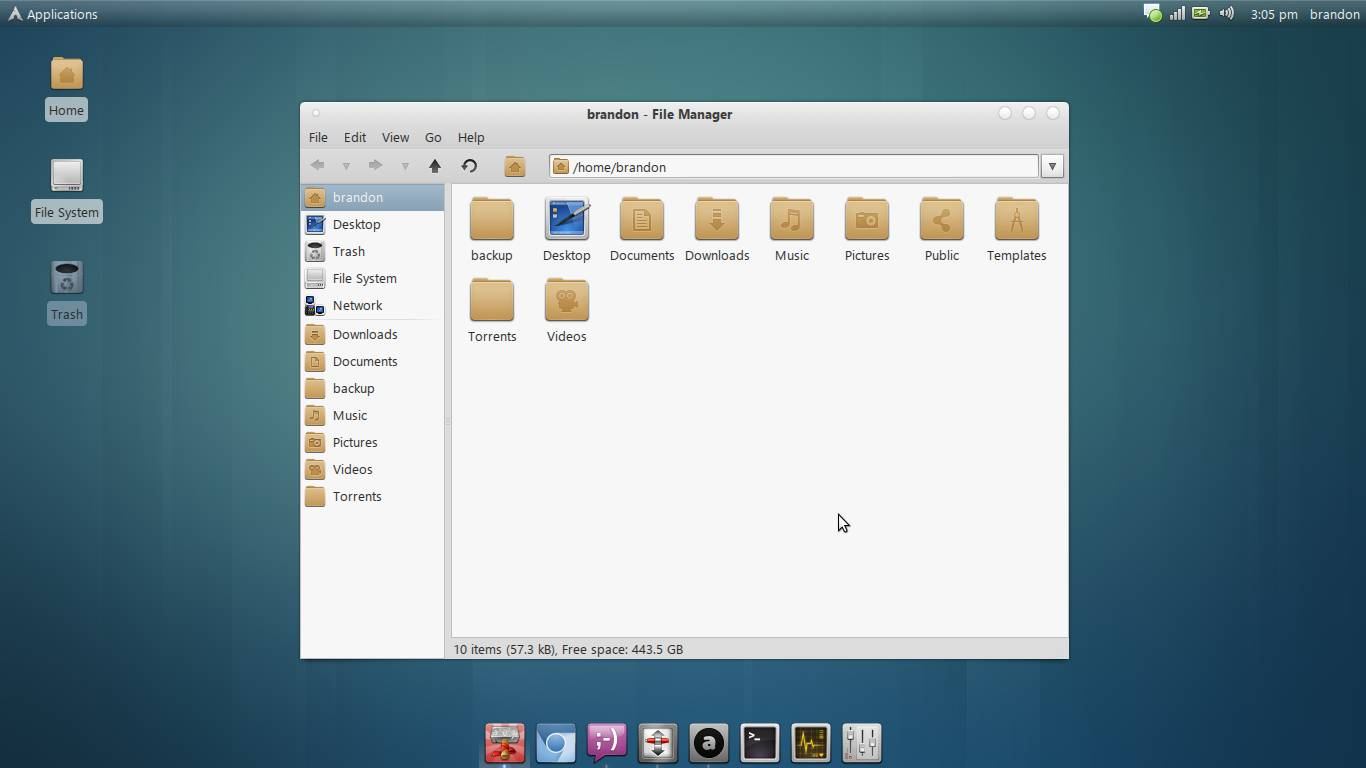
\includegraphics[width=12cm]{XFCE-Desktop}};
    \end{tikzpicture}

\end{frame}

\begin{frame}{Cinnamon}
    \subsubsection{Cinnamon}\label{subsubsec:Cinnamon}

    \begin{tikzpicture}
        [remember picture, overlay, shift={(current page.north east)}]
        \node[anchor=north east,xshift=-0.3cm,yshift=-1.7cm]{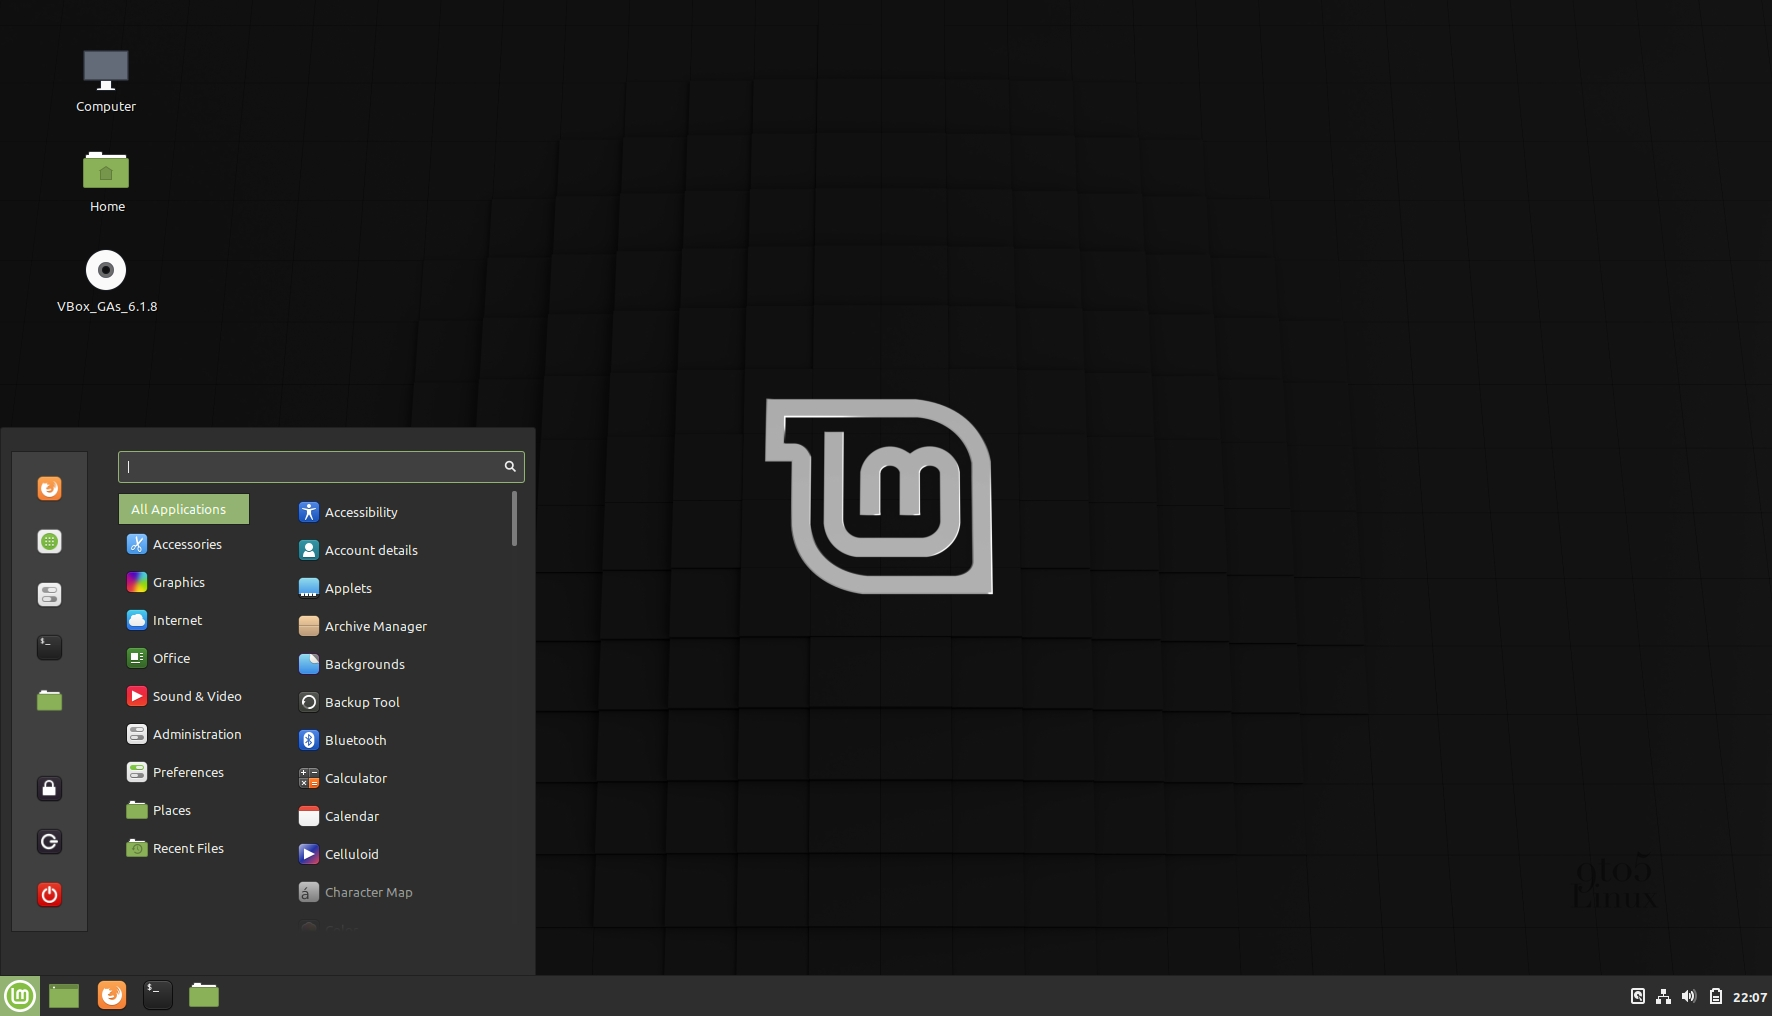
\includegraphics[width=12cm]{Mint-Desktop}};
    \end{tikzpicture}

\end{frame}


% Sources: https://www.forbes.com/sites/jasonevangelho/2019/02/14/5-gorgeous-examples-of-truly-customized-linux-desktops/
% Sources: https://github.com/vinceliuice/McMojave-kde
\begin{frame}{Other Desktops}
    \subsubsection{Other}\label{subsubsec:other}

    \begin{tikzpicture}
        [remember picture, overlay, shift={(current page.north east)}]
        \node[anchor=north east,xshift=-0.3cm,yshift=-1.7cm]{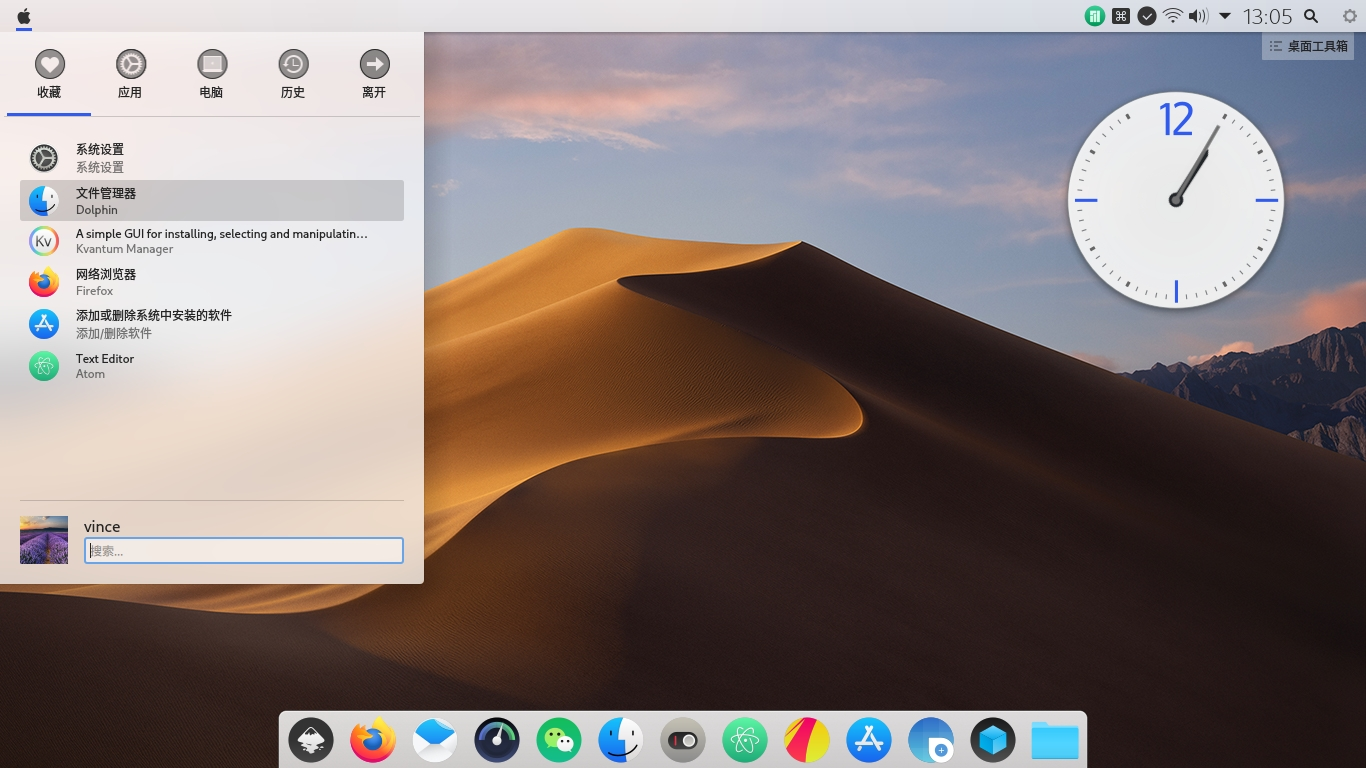
\includegraphics[width=12cm]{KDE-Desktop-MacOS}};
    \end{tikzpicture}

\end{frame}
\begin{frame}{Other Desktops}

    \begin{tikzpicture}
        [remember picture, overlay, shift={(current page.north east)}]
        \node[anchor=north east,xshift=-0.3cm,yshift=-1.7cm]{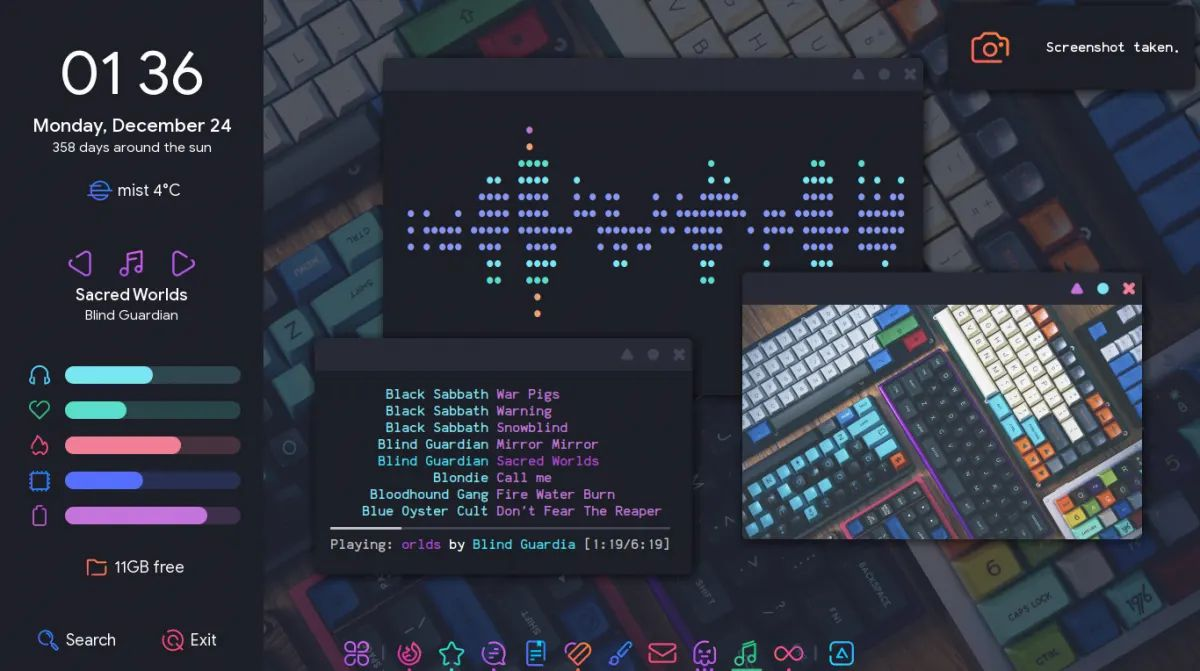
\includegraphics[width=12cm]{other-desktop-1}};
    \end{tikzpicture}

\end{frame}
\begin{frame}{Other Desktops}

    \begin{tikzpicture}
        [remember picture, overlay, shift={(current page.north east)}]
        \node[anchor=north east,xshift=-0.3cm,yshift=-1.7cm]{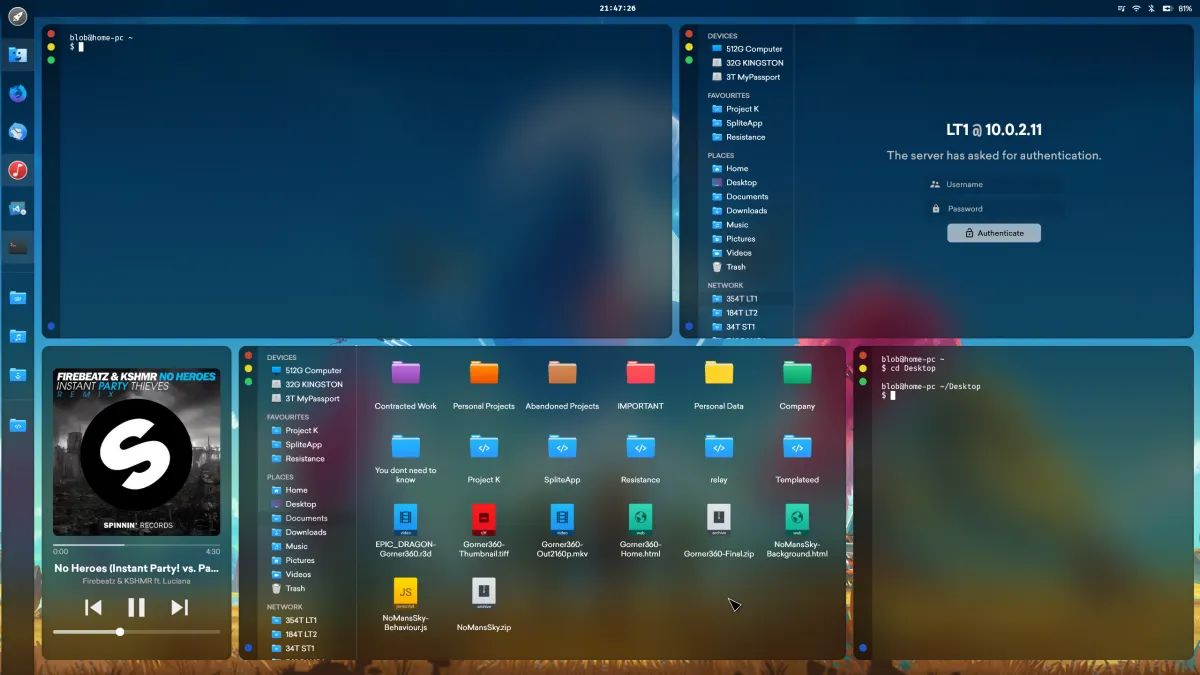
\includegraphics[width=12cm]{other-desktop-2}};
    \end{tikzpicture}

\end{frame}
\begin{frame}{Other Desktops}

    \begin{tikzpicture}
        [remember picture, overlay, shift={(current page.north east)}]
        \node[anchor=north east,xshift=-0.3cm,yshift=-1.7cm]{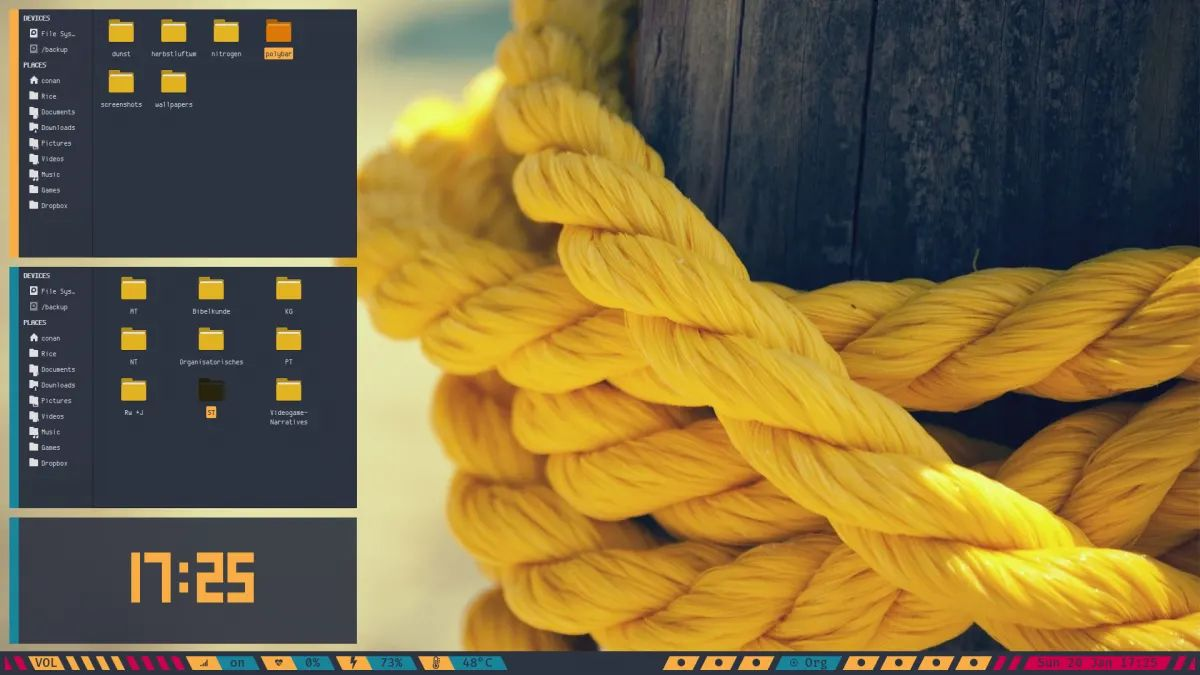
\includegraphics[width=12cm]{other-desktop-3}};
    \end{tikzpicture}

\end{frame}